\chapter{Implementazione del sistema}\label{implementazione}
L'implementazione viene costruita su una serie di framework e librerie di supporto, scelte accuratamente tra le più comuni e potenti usate dalle grandi software house. Il sistema è monolitico e consiste in un'unica applicazione server-side basata su Spring Boot (\url{https://spring.io/projects/spring-boot}). Sia gli amministratori sia gli utenti finali accedono a un'unica istanza del sistema tramite un web browser di propria scelta. In supplemento a tale framework vengono usate le sue estensioni Web, Security e Data (Data JPA) per rendere più facile, leggibile ed efficiente il codice rispettivamente negli ambiti del servlet, della gestione della sessione web e delle credenziali e nella gestione della persistenza. La persistenza è implementata in un database PostgreSQL (si veda il paragrafo \ref{db}) con il supporto della libreria Hibernate. Per quanto riguarda il front-end, l'interfaccia utente viene implementata tramite il framework Vaadin (si veda il paragrafo \ref{gui}). Il sistema comprende file e script di supporto per facilitare il setup all'amministratore di sistema.

Per quanto riguarda la qualità del codice, viene usato un modello \emph{Model, View, Controller} (MVC): model e view risiedono negli omonimi pacchetti Java, mentre il controller è implementato in parte lato model e in parte lato view. L'utilizzo dei design pattern è documentato al paragrafo \ref{pattern}. Il codice è testato tramite piattaforma JUnit (si veda il paragrafo \ref{testing}). Sono inoltre presenti vincoli implementati con \emph{assert}, come spiegato al paragrafo \ref{vincoli}. Viene tenuta traccia delle operazioni del sistema tramite la libreria di logging SLF4J (si veda il paragrafo \ref{logging}).

Le operazioni di compilazione, installazione, esecuzione, soluzione delle dipendenze e in generale di \emph{build} sono gestite dal \emph{build tool} Apache Maven (\url{https://maven.apache.org}). Il progresso del progetto è ovviamente tracciato dal \emph{versioning tool} Git (\url{https://git-scm.com}).




\section{Diagramma di deployment}\label{deployment}




\section{Vincoli}\label{vincoli}
Per i vincoli sul mantenimento della correttezza della rappresentazioni delle classi, si è scelto di usare un metodo equivalente ai vincoli OCL, ma moderno e più funzionale, e che ha un meccanismo di controllo simile a quello di JML. Questo metodo ha delle forti basi teoriche ed è stato introdotto da Barbara Liskov in \emph{Program Development in Java} con il concetto di invariante di rappresentazione: una funzione che restituisce un booleano corrispondente al valore di correttezza dello stato corrente della classe. Questa funzione viene effettivamente implementata nel linguaggio nei metodi \verb!repOk! (\emph{representation ok}) delle varie classi. Con le versioni successive di Java, il metodo ha raggiunto la sua vera potenzialità grazie al meccanismo delle asserzioni: se attivate a runtime (come impostazione della JVM), queste verificano la verità di un booleano e, se falso, sollevano un \verb!AssertionError!. Il metodo consiste quindi in asserire, dopo ogni modifica allo stato dell'istanza (e dopo la costruzione), il valore di \verb!repOk!. Questo permette di controllare in modo automatico, durante l'utilizzo proprio del sistema oppure il testing, che l'invariante rimanga intatto. Alle figure \ref{OCL-VP} (OCL), \ref{JML-VP} (JML), \ref{repOk-VP} (repOk) è rappresentata l'equivalenza dei tre metodi, per il caso rappresentativo della classe \verb!VotingPaper!. I metodi \verb!repOk! sono stati implementati nella branch \emph{constraints}.

\begin{figure}
	\centering
	\begin{verbatim}
context VotingPaper inf:
title<>null and choices<>null and votes<>null and method<>null and hasVoted<>null
and
(method<>ElectionMethod.PREDERENCED implies choices.values()->forAll(sub|sub<>null))
and
votes->forAll(v|v.getMethod()=method)
and
hasVoted->forAll(p|p.canVote()=false)
and
hasVoted->Size()=votes->Size()
        \end{verbatim}
	\caption{OCL di invariante per VotingPaper}\label{OCL-VP}
\end{figure}

\begin{figure}
	\centering
	\begin{verbatim}
/@ invariant
title != null && choices != null && votes != null
                     && method != null && hasVoted != null
&& (\forall VotingPaper sub; choices.values().contains(sub);
        method==ElectionMethod.PREFERENCED ==> sub != null)
&& (\forall Votes v; vote.contains(sub);
        v.getMethod() == method)
&& (\forall Person p; hasVoted.contains(p);
        p.cantVote() == false)
&& hasVoted.size() == votes.size();
@/
        \end{verbatim}
	\caption{JML di invariante per VotingPaper}\label{JML-VP}
\end{figure}

\begin{figure}
	\centering
	\begin{verbatim}
boolean repOk() {
        if (title == null && choices == null && votes == null
                             && method == null && hasVoted == null)
                return false;
        if (method != ElectionMethod.PREFERENCED)
                for (VotingPaper sub : choices.values())
                        if (sub != null)
                                return false;
        for (Vote v : votes)
                if (v.getMethod() != method)
                        return false;
        for (Person p : hasVoted)
                if (!canVote(p))
                        return false;
        return hasVoted.size() == votes.size();
}
        \end{verbatim}
	\caption{repOk per VotingPaper}\label{repOk-VP}
\end{figure}




\section{Testing}\label{testing}
Per il testing viene utilizzato il paradigma del test unitario (\emph{unit testing}) tramite la piattaforma JUnit (\url{https://junit.org/junit5}). Per scelta di design, il codice ha una struttura dichiarativa, con poche strutture di controllo; tuttavia quando applicabile viene usato il criterio di copertura delle decisioni (\emph{decision coverage}), che permette di verificare che il sistema si comporti nel modo previsto nei casi principali, cioè quelli che determinano l'esito di ogni decisione. Nei casi in cui questo non sia sufficiente sono forniti test case supplementari che coprano le singole condizioni (\emph{condition coverage}) all'interno delle decisioni.




\section{Diagramma delle classi di programma}\label{implclassi}
Durante la fase di progettazione, è stato deciso di definire in modo formale la struttura delle classi (come riportato nel diagramma delle classi di progetto alla figura \ref{fig:classdiag}) per definire lo scheletro su cui basare l'implementazione del sistema.
Oltre alla scelta di fornire una struttura rigida, si è deciso anche di non progettare a priori e non fornire vincoli sull'implementazione delle singole classi per due motivi principali.

Il primo riguarda l'agilità nello sviluppo: sfruttando un'infrastruttura rigida, ma con un margine di flessibilità al suo interno, si riesce ad ottenere il vantaggio di una progettazione rigida senza dover rinunciare al vantaggio implementativo dell'adattare il codice all'interno di una classe alle esigenze che derivano dall'implementazione.
Il secondo riguarda la scelta di utilizzo di alcuni framework necessari per la creazione di un prodotto serio e professionale, quali Spring Security e Vaadin. Nonostante lo studio svolto a priori in modo da avere già le conoscenze base necessarie, l'unico modo per comprendere a pieno l'utilizzo di questi strumenti è inevitabilmente tramite lo sviluppo, e questo non era compatibile con una progettazione approfondita e dettagliata sin dalle prime fasi.

In ogni caso, per permettere una piena comprensione del codice sorgente, all'interno di questa relazione è riportato anche il diagramma delle classi di programma (figura \ref{fig:programclassdiag}), al quale è affidato uno sguardo più implementativo.

\begin{figure}[ht]
	\centering
	\includegraphics[width=\textwidth]{UML/programclass.eps}
	\caption{Diagramma delle classi.}
	\label{fig:programclassdiag}
\end{figure}


\section{Design pattern}\label{pattern}


\subsection{Pattern GoF}\label{GoF}
L'utilizzo dei design pattern è massiccio sia nel codice del sistema in sé, sia nell'utilizzo implicito dei framework di supporto. Tra gli utilizzi notevoli:
\begin{description}
	\item[Singleton] la classe \verb!Session! implementa il design pattern: l'unico costruttore della classe è privato e il metodo statico \verb!getSession! fornisce l'unica istanza esistente (se precedentemente istanziata con \verb!initializeSession!) di \verb!Session!. Non è quindi possibile istanziare più di una \verb!Session! contemporaneamente;
	\item[Model-View-Controller (MVC)] i pacchetti \verb!model! e \verb!view! consistono nelle omonime componenti del design pattern; la parte di controller è in parte codificata nella logica sia di \verb!model! sia di \verb!view!, in parte è astratta dall'utilizzo dei framework Vaadin e Spring. Tali framework sono infatti pesantamente fondati sul pattern MVC;
	\item[Data Access Object (DAO)] l'utilizzo della libreria di Spring Data JPA permette di astrarre le classi DAO usate dietro le quinte, tuttavia una loro versione astratta rimane nelle interfacce che estendono \verb!JpaRepository!, che consistono proprio in una serie di operazioni sui dati persistenti che vengono poi implementate automaticamente e fornite agli utilizzatori tramite l'annotazione \verb!@Autowired!. Anche la libreria Hibernate contribuisce all'implementazione dei DAO costruendo query ottimizzate per il database in utilizzo;
	\item[Observer] l'interfaccia costruita da Vaadin è fondamentalmente basata sul pattern observer. Al fine di rendere interattive le pagine senza delegare al programmatore il compito di analizzare il comportamento diretto dell'utente nei confronti del browser, esiste uno strato intermedio che si occupa di notificare i click e le interazioni dell'utente ai componenti interessati. Questo permette una gestione più leggera dell'interfaccia, per migliorare performance e organizzazione del codice sottostante. Eventi come i click e i cambi di pagina vengono notificati dai publisher implementati da Vaadin e vengono ascoltati dai subscriber inseriti durante la creazione dei componenti interattivi delle pagine, i \emph{listener} (per esempio \emph{click listener}), oppure dalla logica intrinseca di Spring Web (ad esempio per il cambio di pagina). Altri esempi sono l'implementazione di \verb!BeforeEnterObserver! nell'interfaccia per il login o l'\verb!@EventListener! utilizzato nella classe \verb!SVeSE! per effettuare operazioni di inizializzazione appena ricevuta la notifica di avvenuto avvio da parte di Spring Boot.
	\item[Service] numerose classi service vengono usate dai framework utilizzati, in aggiunta alle quali alcune sono state costruite specificamente per il sistema SVeSE, specificamente nel pacchetto \verb!security!: la classe \verb!SVeSEUserDetailsService! consiste in un'implementazione dell'interfaccia \verb!UserDetailsService!, usata da Spring Security nell'operazione di login per recuperare i dati sull'utente che viene autenticato; la classe \verb!SecurityService! consiste in una serie di metodi di utility per interagire con la sessione web (per esempio per il logout);
	\item[Adapter] la configurazione della sicurezza web è operata dalla classe \verb!SecurityConfig!, che implementa l'adattatore tra Vaadin e Spring \verb!VaadinWebSecurityConfigurerAdapter!, il cui semplifica le chiamate ai metodi delegandole poi a chiamate di Spring Security;
	\item[Strategy] nel modello, a ogni scheda elettorale è associato un \verb!VoteDecider!, un'interfaccia che si compone di un metodo \verb!canVote! dedicato a discriminare chi ha diritto al voto per la scheda associata. Questa interfaccia implementa il design pattern strategy, dal momento che il diritto di voto della persona può essere determinato da qualunque suo dato, a seconda delle implementazioni dell'interfaccia stessa;
	\item[Iterator] alcune classi del modello implementano l'interfaccia \verb!Iterable!, cioè forniscono un \verb!Iterator!: la scheda elettorale (\verb!VotingPaper!) permette di iterare tra le possibili scelte che essa contiene; la classe \verb!Results! permette di iterare tra i risultati delle singole scelte (\verb!Result!). È comunque molto comune l'utilizzo degli \verb!Iterator!, inclusi quelli forniti dalla libreria standard di Java.
\end{description}


\subsection{Pattern GRASP}
L'attenzione ai principi GRASP (\emph{General Responsibility Assignment Software Patterns}) è costante durante lo sviluppo.
\begin{description}
	\item[High Cohesion] ogni classe, con pochissime eccezioni, ha una sua coerenza semantica, dal momento che rappresenta un oggetto o concetto reale (sessione di voto, scheda elettorale, etc.);
	\item[Low Coupling] i collegamenti tra classi mettono in relazione oggetti semantici diversi tra loro, mentre gli aspetti coesi sono raggruppati nella stessa classe (una sessione ha alcune schede elettorali);
	\item[Information Expert] i campi delle classi sono organizzati in modo da mantenere l'informazione a chi appartiene alla corretta area semantica, di modo che l'\emph{information expert} non confligga con il principio di coesione;
	\item[Creator] ad eccezione dei casi in cui il costruttore è una scelta migliore, la costruzione della classe è delegata a chi ne ha la responsabilità (ad esempio il metodo statico per il \emph{singleton} \verb!Session!);
	\item[Controller] si veda MVC al paragrafo \ref{GoF};
	\item[Polymorphism] interfacce come \verb!Vote! e \verb!VoteDecider! garantiscono di poter usare diverse implementazioni pur mantenendo valida la funzionalità;
	\item[Pure Fabrication] le poche classi di pura invenzione mantengono un'area semantica coesa. Si veda anche Service al paragrafo \ref{GoF};
	\item[Indirection] l'utilizzo di classi di supporto alla comunicazione è volutamente limitato ai fini di minimizzare il \emph{coupling}, tuttavia è presente ad esempio negli adapter (paragrafo \ref{GoF});
	\item[Protected Variations] l'utilizzo delle interfacce e in generale la buona pratica di usare tipi apparenti in alto nella gerarchia, oltre che ovviamente l'utilizzo di getter e setter invece di dare visibilità ai campi, permette la modifica futura delle implementazioni pur mantenendo la funzionalità del sistema.
\end{description}




\section{Interfaccia grafica}\label{gui}

\subsection{Introduzione e linee guida}
Nello studio delle scelte da prendere per quanto riguarda la progettazione dell'interfaccia grafica, è stato fatto riferimento al documento ministeriale. Citando testualmente l'Art.2 Comma 2: \emph{"Il sistema di voto elettronico dovrebbe basarsi su webapplication, conforme ai requisiti di usabilità e accessibilità previsti dalla legge [...]"}. 
Per questo motivo, il primo principio che ha guidato l'implementazione è stata la decisione di utilizzare un framework che ci permettesse di creare agilmente una webapplication: la scelta finale è stata Vaadin.
La seconda linea guida è stata una scelta di stile dell'interfaccia, in modo che risultasse il più chiara possibile. Per questo motivo sono stati utilizzanti componenti grafici estremamente semplici (come bottoni e caselle di testo), limitando la complessità dell'interfaccia.
Per migliorare l'accessibilità sono stati integrati anche alcuni pop-up di conferma (vedi fig. \ref{screeenshot:newsessionconfirm}) per confermare le operazioni più importanti.
\begin{figure}
	\centering
	
\includegraphics[width=0.5\textwidth]{img/gui/newSessionConfirm.png}
	\caption{Pop-up di conferma nella creazione di una nuova sessione}
	\label{screeenshot:newsessionconfirm}
\end{figure}

\subsection{Barra di navigazione}
In ogni interfaccia è presente una barra di navigazione collocata nella parte altra dello schermo: essa permette di navigare tra le varie tab dell'applicazione con facilità, ed è customizzata in base al ruolo dell'utente loggato nell'applicazione. 
Nel caso in cui l'applicazione sia utilizzata dall'admin, all'interno della barra di navigazione sono presenti i riferimenti alle viste utilizzabili dall'amministratore di sessione mentre invece nel caso in cui sia un garante ad essere loggato, la barra è diversa (vedi fig. \ref{screenshot:mainview}).
\begin{figure}
	\centering
	
\includegraphics[width=0.45\textwidth]{img/gui/adminMainView.png}
	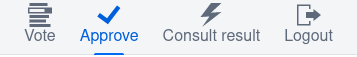
\includegraphics[width=0.45\textwidth]{img/gui/guarantorsMainView.png}
	\caption{Barra di navigazione di un admin (sx) e di un garante (dx)}
	\label{screenshot:mainview}
\end{figure}

\subsection{Login}
Anche la schermata di login è penstata per essere intuitiva, con un singolo riquadro dove inserire le proprie credenziali, e un messaggio di errore contrassegnato dal colore rosso, per aiutare la comprensione anche a persone con difficoltà nel leggere le scritte (vedi fig. \ref{screenshot:login}

\begin{figure}
	\centering
	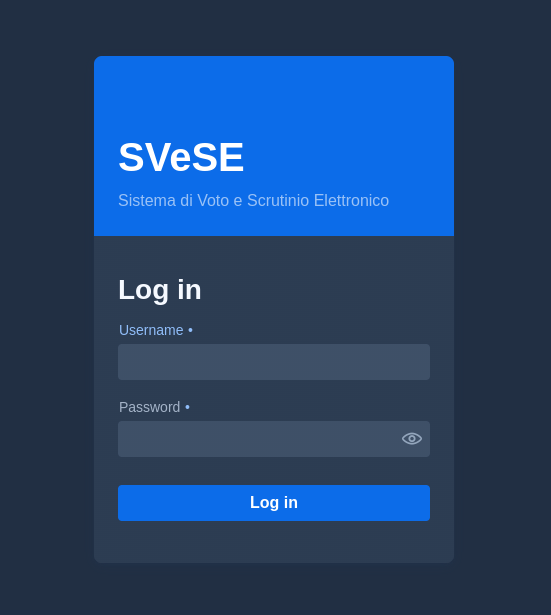
\includegraphics[width=0.4\textwidth]{img/gui/login.png}
	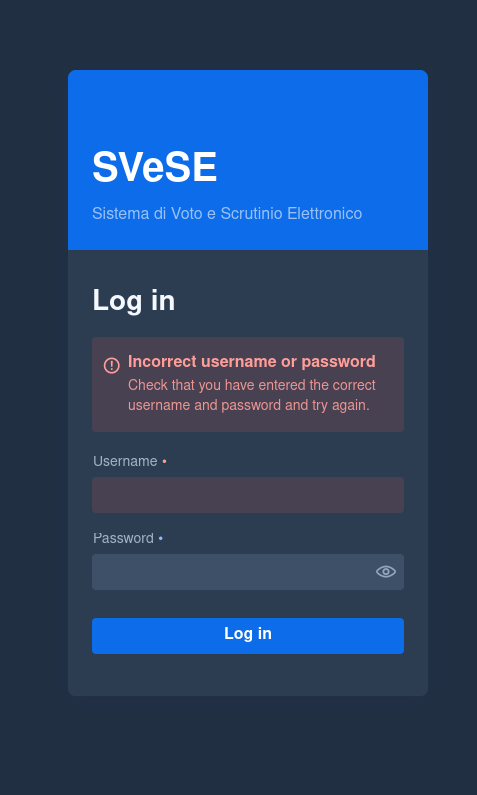
\includegraphics[width=0.4\textwidth]{img/gui/loginError.png}
	\caption{Modulo di login all'avvio dell'applicazione e dopo l'inserimento errato delle credenziali}
	\label{screenshot:login}
\end{figure}

\subsection{Menu di voto}
I menu di voto possono essere di due tipi, collegati al metodo di voto della scheda. Dopo aver scelto la scheda tramite un bottone, viene mostrata una scelta multipla nel caso in cui il voto da esprimere sia categorico, mentre nel caso in cui il voto sia ordinale, viene proposta una serie di menu a tendina, utilizzabili per selezionare l'ordine (vedi fig \ref{screenshot:vote}).

\begin{figure}
	\centering
	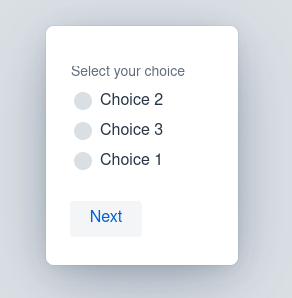
\includegraphics[width=0.4\textwidth]{img/gui/categoricalVoting.png}
	\includegraphics[width=0.4\textwidth]{img/gui/OrdinalVoting.png}
	\caption{Menu di voto nel caso di una scheda con voto categorico (sx) e con voto ordinale (dx)}
	\label{screenshot:vote}
\end{figure}

\subsection{Creazione di una nuova sessione}
L'interfaccia più complessa è l'interfaccia per la creazione di una nuova sessione: il motivo è che questa operazione richiede un elevato numero di informazioni, come data di inizio e fine, schede elettorali presenti con relative scelte e metodi\ldots 
In questo caso però la complessità è un problema ridotto, perchè questa interfaccia è utilizzabile solamente dall'amministratore, che si suppone abbia un buon grado di confidenza con il sistema.
I vari componenti non hanno bisogno di ulteriore presentazione, perchè sono tutti accompagnati da una casella di testo che ne spiega la funzione (vedi fig \ref{screenshot:newsession}). L'unica nota è che la checkbox "Suboptions", utilizzata per creare schede con \emph{voto categorico con preferenze}, apre un'interfaccia analoga a quella della creazione della scheda principale.

\begin{figure}
	\centering
	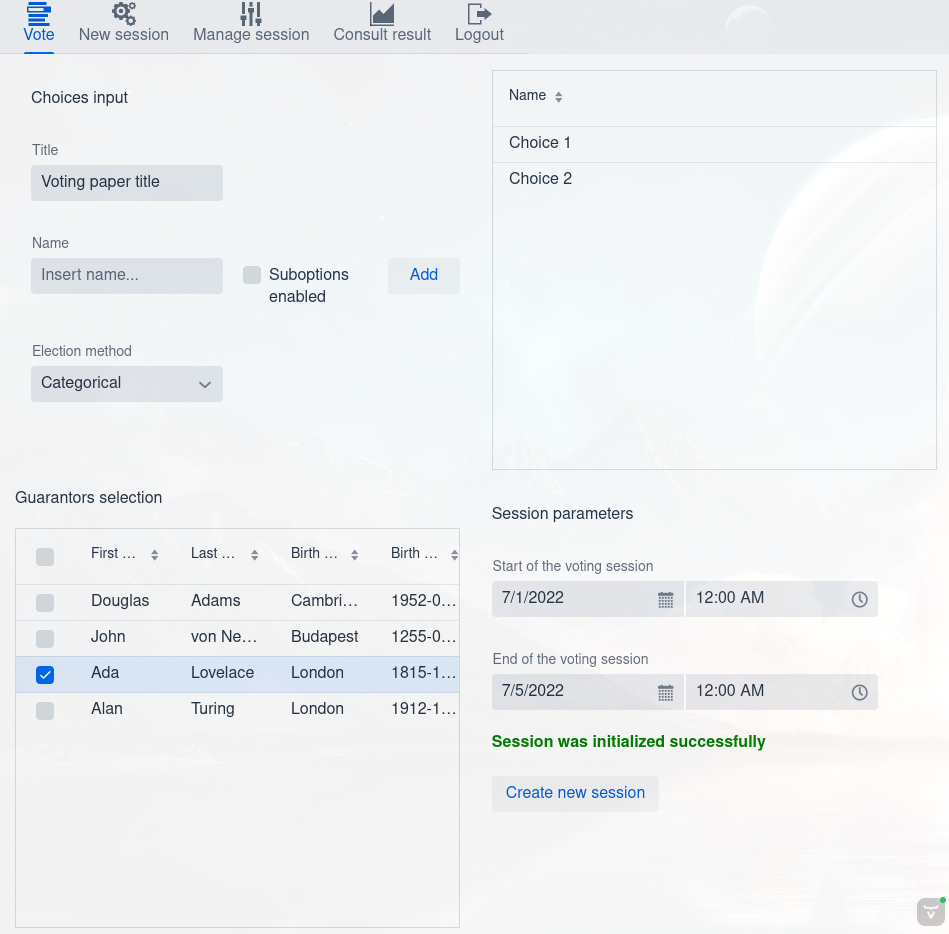
\includegraphics[height=0.8\textwidth, angle=90]{img/gui/newSession.png}
	\caption{Interfaccia per la creazione di una nuova sessione di voto}
	\label{screenshot:newsession}
\end{figure}

\subsection{Consultazione risultati}
L'interfaccia di consultazione dei risultati è anch'essa suddivisa in due modalità, una per le schede con voto categorico, categorico con preferenze e referendum, l'altra per le schede con voto ordinale. (vedi fig. \ref{screenshot:consultresult}). Nel caso del voto categorico con preferenza, è possibile consultare separatamente il voto delle schede secondarie.
Anche in questo caso per consultare i risultati è sufficiente cliccare sul bottone della scheda corrispondente.

\begin{figure}
	\centering
	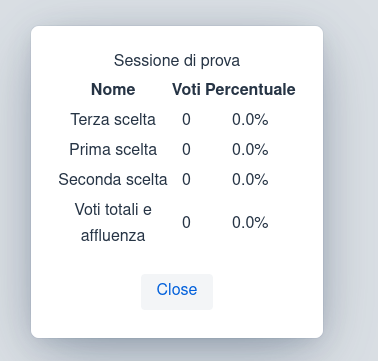
\includegraphics[height=0.3\textwidth]{img/gui/consultResult.png}
	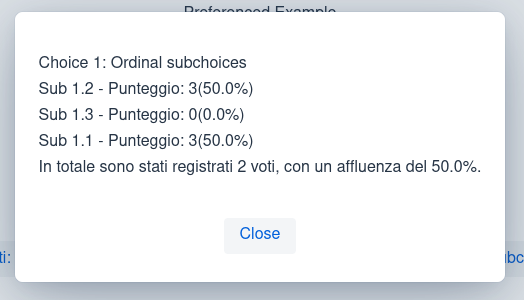
\includegraphics[height=0.3\textwidth]{img/gui/consultResultOrdinal.png}
	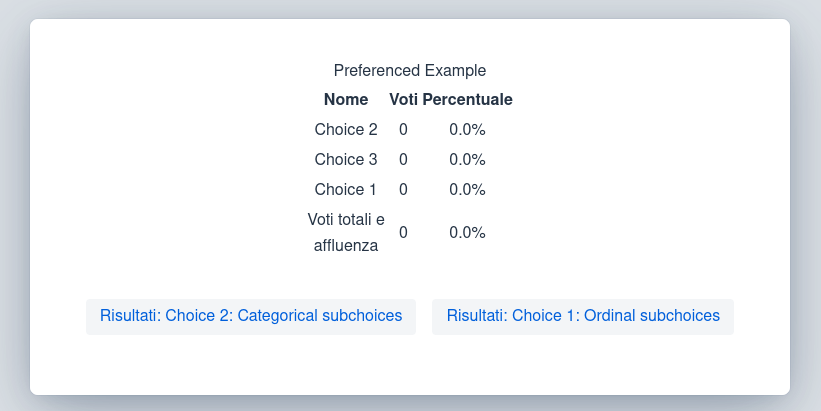
\includegraphics[height=0.4\textwidth]{img/gui/consultResultPreferenced.png}
	\caption{Interfaccia per la consultazione dei risultati di una sessione di voto}
	\label{screenshot:consultresult}
\end{figure}


\section{Persistenza dei dati}\label{db}
I dati persistenti sono memorizzati in un database PostgreSQL (\url{https://www.postgresql.org}) e gestiti tramite l'interfaccia JPA (Java Persistent API, standard introdotto da Oracle) implementata da Spring Data. La gestione è supplementata dall'utilizzo di Hibernate (\url{https://hibernate.org}), una libreria che ottimizza la gestione della persistenza e costruisce automaticamente query SQL pensate per un certo \emph{dialetto}, cioè specifiche per un DBMS. Spring Data permette di programmare servizi DAO come interfacce Java (repository) in cui i metodi hanno nomi significativi, che poi vengono implementate automaticamente dal framework. Grazie a questa astrazione, le query SQL sono ottimizzate e versatili (non \emph{hard-coded}); è possibile infatti cambiare, se lo si volesse, il DBMS con il minimo sforzo, modificando unicamente il file \verb!application.properties!. Le query SQL sono comunque visibili, a meno dei dati sensibili, nei log del sistema.




\section{Auditing}\label{logging}
I framework Spring e Vaadin (descritti in precedenza) contengono un sistema di logging basato sull'interfaccia della libreria SLF4J (\url{https://www.slf4j.org}). Gli eventi generati dai due framework di cui sopra sono quindi loggati automaticamente. Gli eventi del sistema SVeSE, in particolare la logica del modello, sono tracciati da chiamate (aggiunte nel codice) alla medesima libreria, di modo da uniformare l'output e l'archiviazione dei log sotto un'unica configurazione. SLF4J consiste in un'interfaccia che unifica potenzialmente diverse librerie di logging, per cui è molto semplice, con piccole modifiche alla configurazione, adottare il logging nativo di Java oppure, ad esempio, Log4j (\url{https://logging.apache.org/log4j}).




\section{Sicurezza}\label{security}
Anche ai fini di conformità con le direttive ministeriali, il supporto alla sicurezza è affidato alla gestione professionale fornita dal modulo Security del framework Spring. Tale modulo gestisce la sessione web e il login, mentre la persistenza delle utenze è gestita da Spring Data JPA e configurata ad-hoc per il Sistema. Ovviamente non vengono memorizzate password in chiaro, ma i rispettivi hash muniti di salt e generati con l'algoritmo ad alta sicurezza \emph{blowfish}. Grazie al servizio personalizzato di login \verb!SVeSEUserDetailsService!, l'utenza autenticata, che in Spring Security corrisponde a un oggetto \verb!UserDetails!, viene fatta corrispondere a un oggetto \verb!Person! del modello, a cui si può accedere facilmente tramite il metodo \verb!getAuthenticatedPerson! del servizio \verb!SecurityService!. Questo permette di effettuare le dovute operazioni con tutte le informazioni necessarie sulla persona autenticata, determinandone eventuali ruoli speciali (come quello di garante) e prerogative (ad esempio, se può votare per una certa scheda). Il pacchetto \verb!security!, in generale, contiene la configurazione della porzione di sicurezza e la fusione trasparente delle classi di Spring Security con quelle del modello.
